% !TeX spellcheck = da_DK
\chapter{Nervefysiologi}\label{AppNerve}
Kroppens nervesystem kan inddeles i to dele; det centrale nervesystem (CNS) og det perifere nervesystem (PNS). CNS indeholder encephalon og columna, mens PNS indebærer kommunikationen imellem CNS og kroppens øvrige dele. PNS kan yderligere opdeles i det somatiske nervesystem, som består af det motoriske og sensoriske nervesystem, og autonome nervesystem, som består af en sympatisk og parasympatisk del. Det somatiske nervesystem styrer kroppens bevidste bevægelser og sender afferente signaler tilbage til CNS, hvorimod det autonome nervesystem regulerer kroppens ubevidste funktioner. Det er altså PNS, som registrerer signaler, CNS integrerer disse signaler og dirigerer et motorisk signal, som PNS skal omsætte til en handling. \cite{Martini2012,Stanfield2014} Et overblik over dette ses på \figref{Nersys}.

\begin{figure}[H]
	\centering
	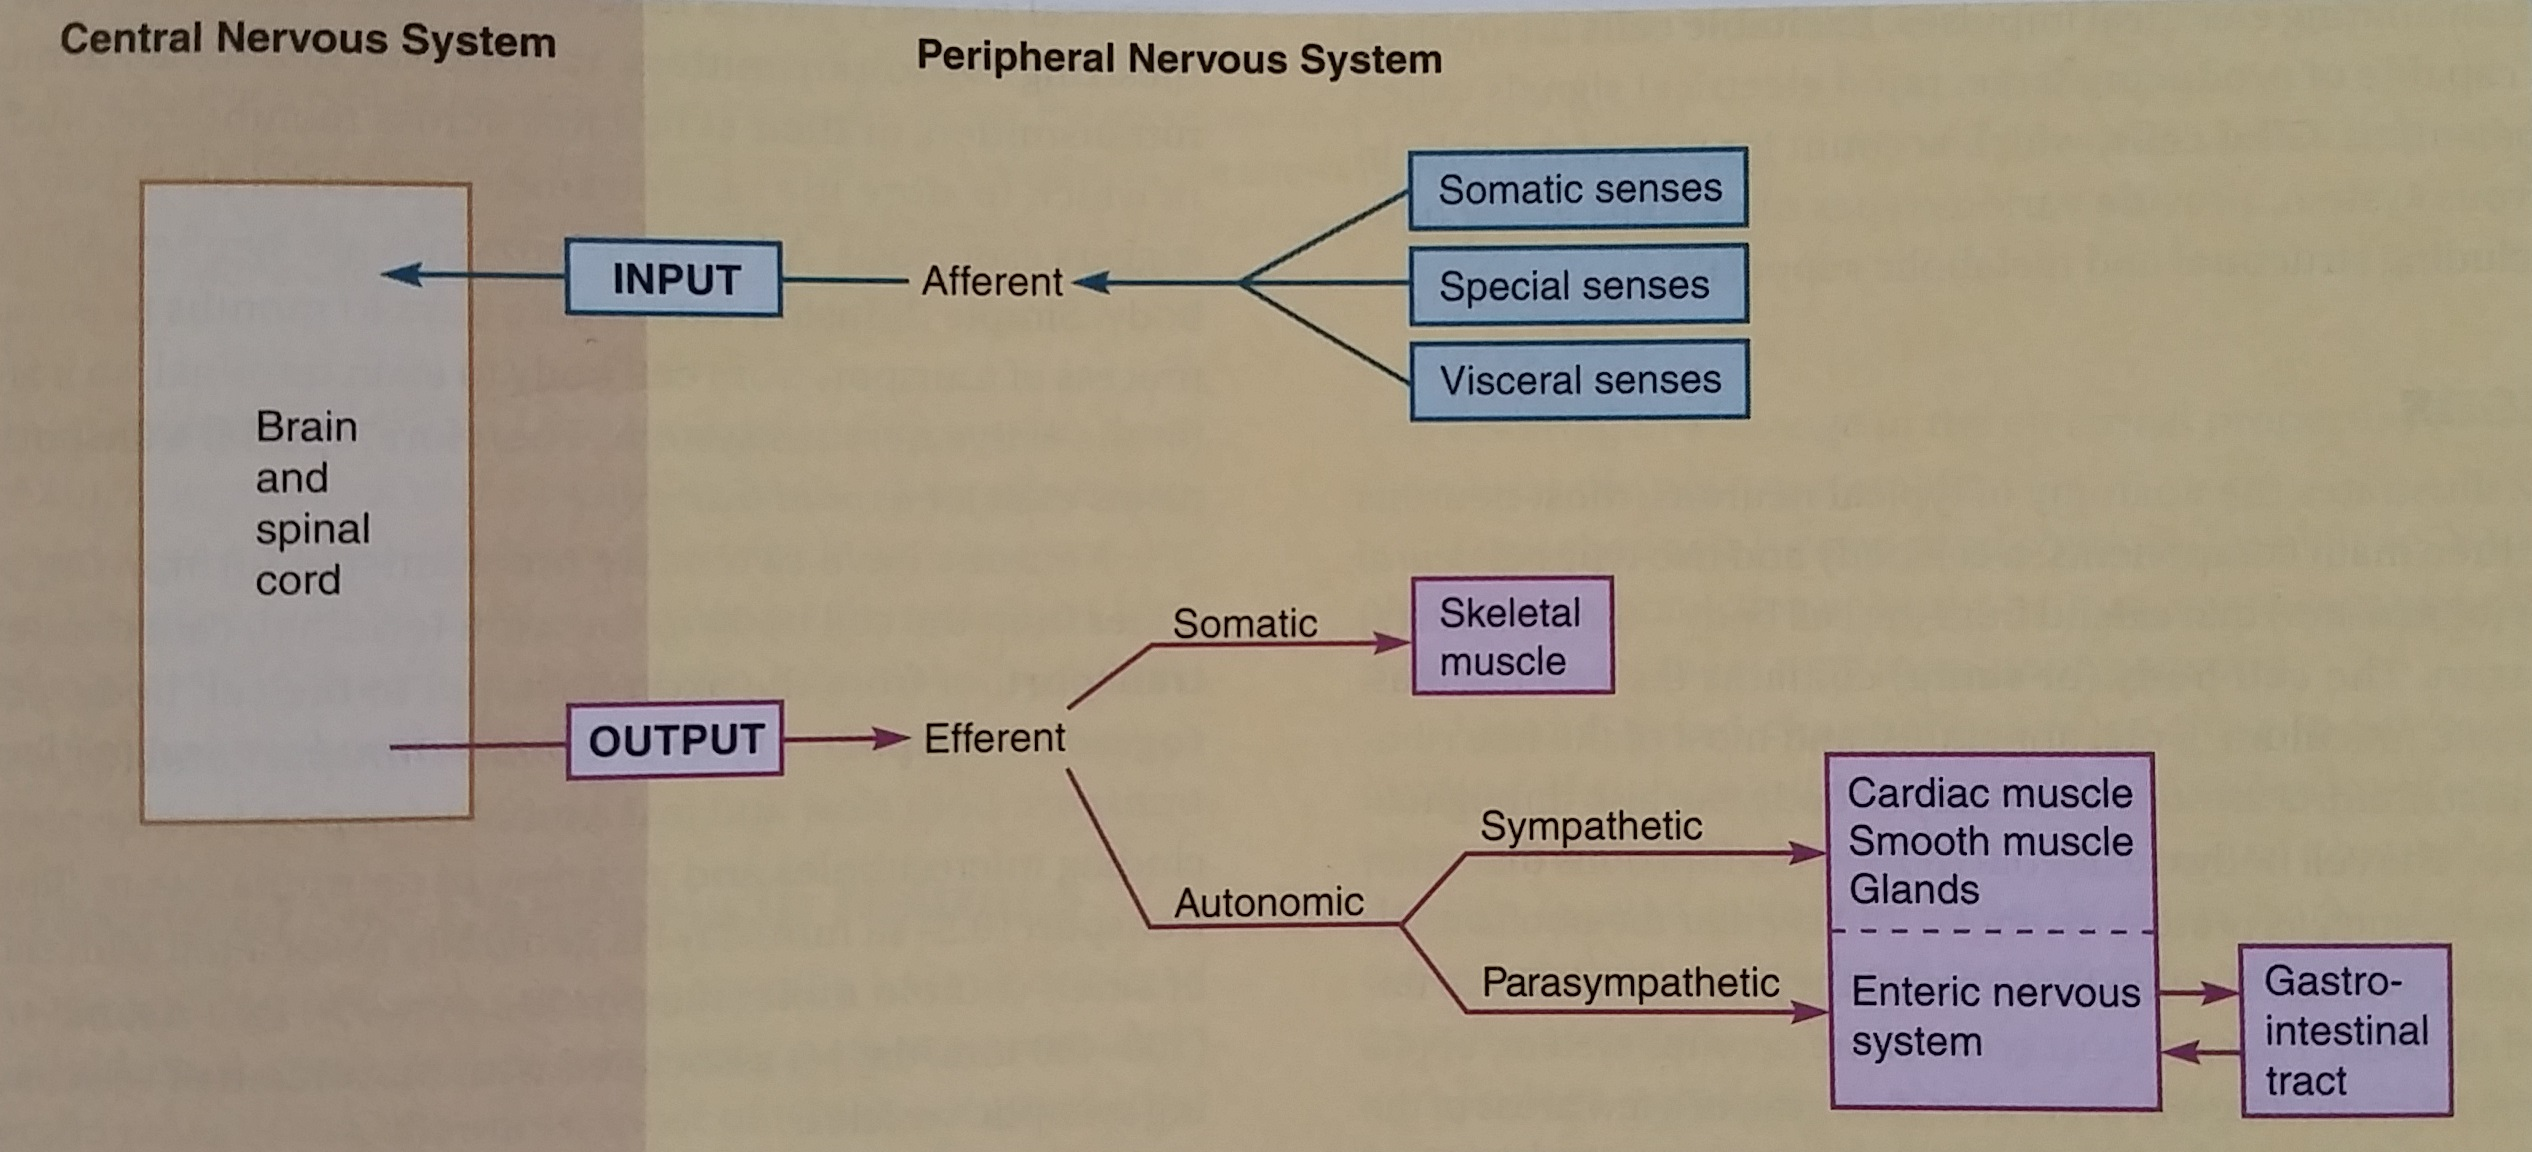
\includegraphics[scale=0.15]{figures/bProblemanalyse/Nervesys1.jpg}
	\caption{På figuren ses en opdeling af PNS og CNS samt hvordan et signal proceseres til en handling af nervesystemerne. \cite{Stanfield2014}}
	\label{Nersys}
\end{figure}

\section{Hjernens anatomi}
Cerebrum er encephalons største del og er involveret i sanseintegration, styring af frivillige bevægelser og højere intellektuelle funktioner, såsom tale og abstrakt tænkning. \cite{Academic2015b} Cerebrums ydre lag hedder cerebral cortex men kaldes hjernens grå substans. Her ligger nervers soma med dendritter. Cerebral cortex har forskellige centre, men kan også inddeles i højre og venstre halvdel. Delen af cerebral cortex, der kontrollerer kroppens motorik med motor cortex, kaldes gyrus præcentralis. Nerverne i dette område leder motoriske impulser til kroppens muskler igennem nervebanerne i den hvide substans, som indeholder nervernes aksoner og fungerer derved som transportvej. \cite{Academic2015b,Martini2012,Stanfield2014} Disse aksoner krydses i medulla oblongata og medulla spinalis og løber derefter til den modsatte legemeshalvdel fra, hvor impulsen afsendes. \cite{Martini2012}

Når en bevægelse udføres, starter det med en idé eller en intention om at lave en bevægelse. Denne tanke opstår i det præfrontale cortex, som findes i lobus frontalis. Præfrontal cortex er specielt aktivt under udførelse af nye situationer / bevægelser og har forbindelse til motor cortex, som sætter indlærte bevægelser i gang. Samtidig modtager basalganglier i cerebellum signalet, hvorved kroppen kan modificere bevægelsen i forhold til omgivelserne. Cerebellum samarbejder altså med motor cortex, så bevægelsesplanen kan samles og sendes via de decenderende baner i medulla spinalis til bestemmelsesstedet. \cite{Bojsen-Moeller2012} \\
Hvis en bevægelse gentages, vil præmotor cortex gemme stimulationsmønstret. Dette gør, at bevægelsen kan udføres nemmere og mere præcist end ellers. Bevægelsen lagres i basalganglierne ved at synapseforbindelserne er styrket. \cite{Martini2012}

\section{Nervens anatomi}
En nerve består af soma, dendritter og et myelineseret akson. Soma indeholder cellekernen, endoplasmatisk reticulum, golgi apparater og de fleste frie ribosomer. Indholdet i soma bestemmer, hvordan cellen agerer med andre samt dets funktion og vedligeholdelse. Dendritter er udløbere fra soma, som modtager impulser fra en anden nerve og fører signalet ind til cellekroppen. Aksonet leder impulser fra soma til sin ende, der har mange små forgreninger, kaldet aksonterminaler. Disse danner synapser med targetorgan eller andre nervers dendritter. \cite{Stanfield2014} \\
En nerve kan kun lede signaler, hvis der forekommer en tilstrækkelig høj elektrisk spændingsforskel mellem det intracellulær- og ekstracellulærvæske af membranen. Dette danner et aktionspotentiale. I en hvilende nerve er der et overskud af negative ioner i den intracellulære væske i forhold til den ekstracellulære væske. Denne spændingsforskel mellem det intracellulære og ekstracellulære kaldes membranpotentialet. \cite{Martini2012,Stanfield2014}

\section{Aktionspotentiale}
Signaler i kroppen videresendes vha. aktionspotentialer. En celle i hvile har et spændingsniveau på ca. -70 mV, hvilket skyldes koncentrationsforskellen mellem natrium-ion ($Na^{+}$) udenfor cellen og kalium-ion ($K^{+}$) indvendigt i cellen. Begge ioner kan diffundere over cellemembranen, men spændingsniveauet kan stadig opretholdes af natrium/kalium-pumpen. Denne pumpe skaber en ligevægt imellem indpumpning af $K^{+}$ og udpumpning af $Na^{+}$. Hvis en nervecelle modtager et stimulus, påvirker dette mekanisk- eller kemisk styrede $Na^{+}$ kanaler, som vil åbne sig og pumpe mere $Na^{+}$ ind i cellen. Derved stiger permeabiliteten af $Na^{+}$ og den samlede ladning af cellen ændres. Hvis den påbegyndte stimulus, som skaber et gradet potential, ikke var stærk nok til, at cellen når sin tærskelværdi, vil natrium kanalerne lukkes. Natrium/kalium-pumpen vil derefter arbejde sig tilbage til hvile spændingsniveauet. Hvis stimulus var stærkt nok til, at mange natriumkanaler åbner sig og cellen når sin tærskelværdi, så vil de elektrisk styrede natriumkanaler også åbne sig som reaktion på, at spændingsforskellen bliver mindre. Herved ender cellen med et overskud af negativ ladning udenfor ift. indenfor cellemembranen dvs. den modsatte situation af hvile, hvilket skaber et aktionspotentiale. \cite{Martini2012,Stanfield2014}

\begin{figure}[H]
	\centering
	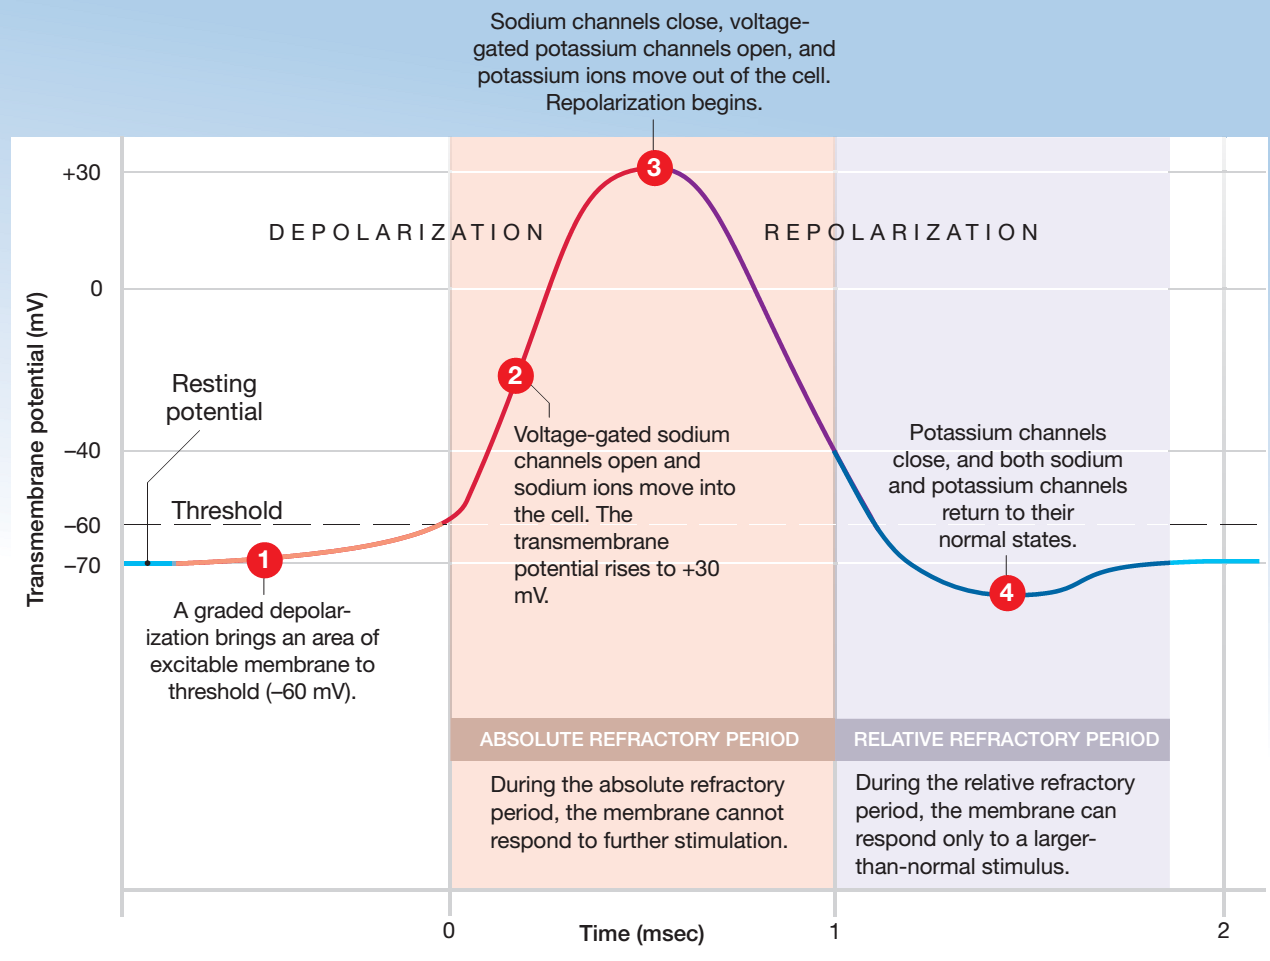
\includegraphics[scale=0.45]{figures/bProblemanalyse/Aktion2.png}
	\caption{På figuren ses stadierne for et aktionspotentiale. \cite{Martini2012}}
	\label{nervemuskel}
\end{figure}

Når et nervesignal skal overføres til en muskel, sker det i en neuromuskulær synapse, som er en kemisk synapse. Den kemiske synapse består generelt af en præsynaptisk terminal, en synapsekløft og en postsynaptisk celle. En vigtig egenskab ved den kemiske synapse er, at aktionspotentialer udelukkende kan bevæge sig i én retning; fra den præsynaptiske terminal imod den postsynaptiske terminal.\cite{Hall2015} Vesiklerne i den præsynaptiske terminal rummer neurotransmittere, som er et kemisk stof, der overfører signalet på tværs af synapsen. I neuromuskulære synapser vil neurotransmitteren ofte være acetylcholin (ACh). Ved et aktionspotentiale vil den præsynaptiske terminal frigive ACh, som bevæger sig ud i synapsekløften mod receptorerne på muskelfiberen. Bindingen af ACh til receptorerne medfører en depolarisering af den synaptiske kløft ved diffusion af $Na^{+}$. Herved bliver aktionspotentialet transporteret ned til sarcoplasmatisk reticulum i muskelfiberen, som frigiver $Ca^{2+}$ til filamenterne i myofibrillerne, der gør kontraktion af musklen mulig.\cite{Hall2015,Martini2012} Dette ses på \figref{nervemuskel}.

\begin{figure}[H]
	\centering
	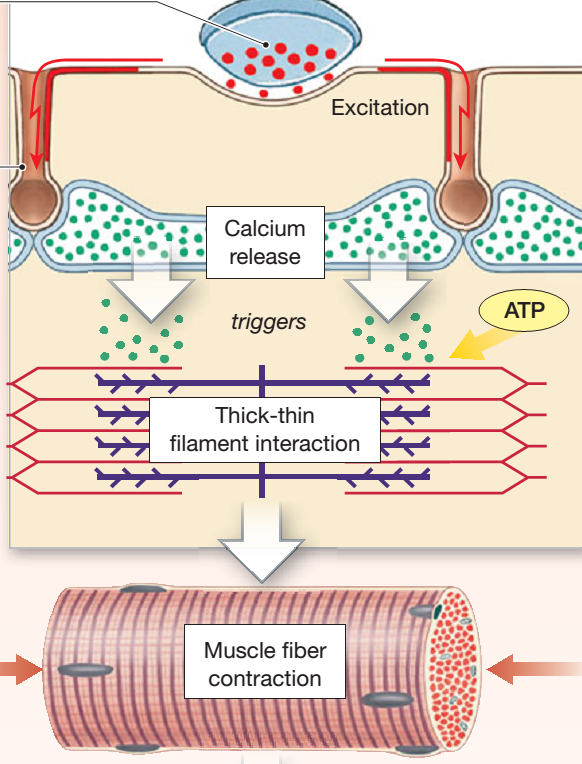
\includegraphics[scale=0.7]{figures/bProblemanalyse/Aktion1.png}
	\caption{På figuren ses, hvordan nervens frigivelse af ACh sætter en muskelkontraktion i gang. \cite{Martini2012}}
	\label{nervemuskel}
\end{figure}